% ACL 2026 long paper (ARR). Compile with pdfLaTeX + BibTeX:
%   latexmk -pdf main.tex      (or Overleaf: upload the whole paper/ folder)
% Red \todo{...} marks writing that is still missing; red \tbd cells mark experiments that have
% not been run yet. Both are indexed in ../PLAN.md (Section 6, E1--E12).
\documentclass[11pt]{article}
\usepackage[review]{acl}
\usepackage{times}
\usepackage{latexsym}
\usepackage[T1]{fontenc}
\usepackage[utf8]{inputenc}
\usepackage{microtype}
\usepackage{inconsolata}
\usepackage{graphicx}
\usepackage{amsmath}
\usepackage{amssymb}
\usepackage{booktabs}
\usepackage{multirow}
\usepackage{enumitem}
\usepackage{xspace}
\usepackage{xcolor}
\usepackage{CJKutf8}
\usepackage{tikz}
\usetikzlibrary{positioning,arrows.meta,fit,backgrounds,calc}

% ---------------------------------------------------------------- macros
\newcommand{\umr}{\textsc{UMR}\xspace}
\newcommand{\amr}{\textsc{AMR}\xspace}
\newcommand{\ours}{decision orchestration\xspace}
\newcommand{\Ours}{Decision orchestration\xspace}
\newcommand{\skill}[1]{\texttt{#1}}
\newcommand{\zh}[1]{\begin{CJK}{UTF8}{gbsn}#1\end{CJK}}
\newcommand{\todo}[1]{\textcolor{red}{[TODO: #1]}}
\newcommand{\tbd}{\textcolor{red}{--}}
\newcommand{\exper}[1]{\textcolor{red}{\textsc{[#1]}}}   % pointer to an experiment in PLAN.md
\newcommand{\F}{F\xspace}

\title{Decision Orchestration:\\
Learning Annotation Procedures from a Handful of Gold Documents}

\author{Anonymous ACL submission}

\begin{document}
\maketitle

\begin{abstract}
Every new annotation scheme starts with a guideline and almost no data. Supervised parsers need thousands of examples, and an LLM prompted with the guideline ignores its conventions, emits malformed output, and cannot be debugged. We observe that a guideline is mostly a procedure: most steps are deterministic, and only a few call for judgment. We propose \emph{decision orchestration}, which compiles a guideline into an executable procedure. Code runs the steps, enforces well-formedness and assembles the output, and a model is consulted only at decision points, for a schema-constrained fragment or for probabilities over the options of a closed question. We then learn the procedure itself, not model weights, from a handful of gold documents. Decision thresholds are calibrated by measurement, uncertain decisions are routed to a stronger model, and reflection attributes each error to the node that made it and keeps an edit only if it measurably helps. On Chinese Uniform Meaning Representation parsing, orchestration lifts a 9B model from 0 to 17.6 F, two gold documents raise a frontier model from 45.3 to 52.6 F, recalibration on four documents adapts a new decision model (+2.9 F), and routing recovers 75\% of a stronger model's gain at 26\% of its cost. \todo{PARSEME sentence once E9 is run}
\end{abstract}

%=====================================================================
\section{Introduction}
\label{sec:intro}

%---------------------------------------------------------------------
\begin{figure*}[t]
\centering
\resizebox{\textwidth}{!}{%
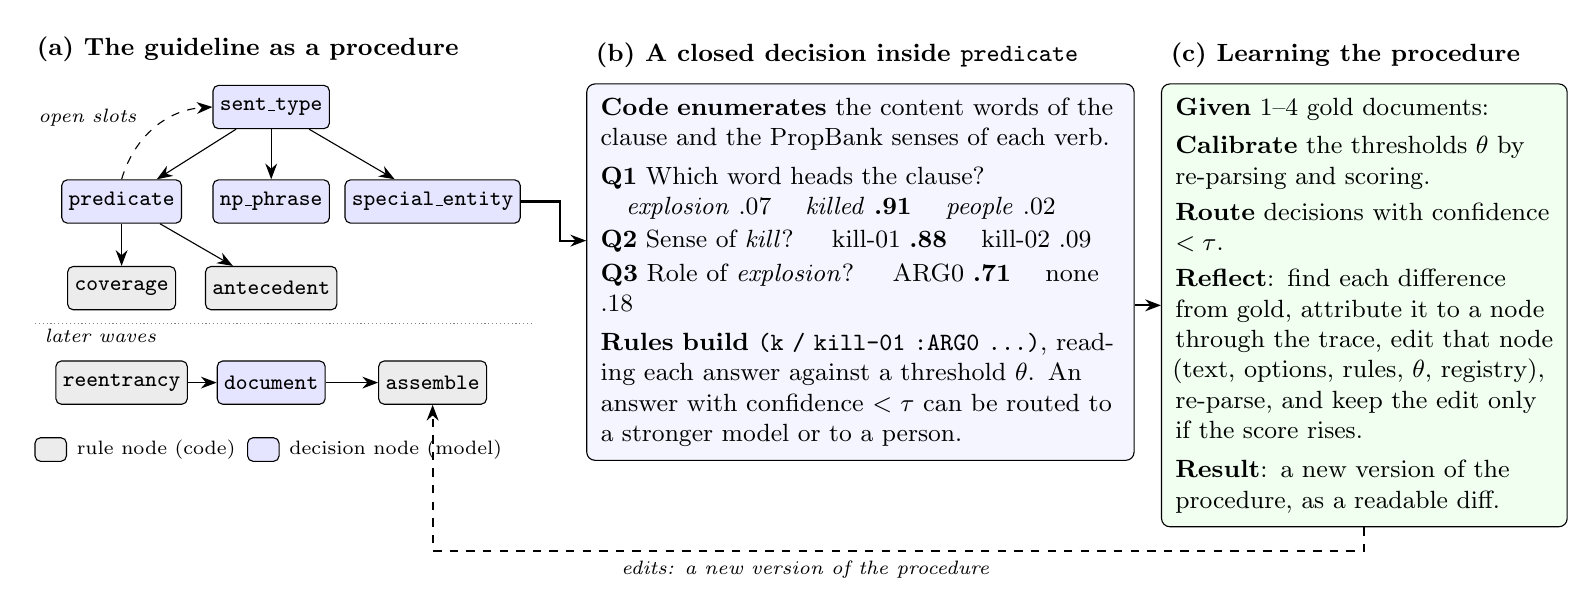
\begin{tikzpicture}[
    font=\small,
    >={Stealth[length=2mm]},
    rule/.style={draw, rounded corners=2pt, fill=gray!15, minimum height=5.5mm, inner sep=2.5pt, font=\footnotesize\ttfamily},
    dec/.style={draw, rounded corners=2pt, fill=blue!10, minimum height=5.5mm, inner sep=2.5pt, font=\footnotesize\ttfamily},
    box/.style={draw, rounded corners=3pt, inner sep=5pt, align=left},
    ttl/.style={font=\small\bfseries, anchor=south west},
  ]
  % ---------------- (a) the procedure
  \node[dec] (st) at (2.6,0) {sent\_type};
  \node[dec] (pr) at (0.7,-1.2) {predicate};
  \node[dec] (np) at (2.6,-1.2) {np\_phrase};
  \node[dec] (se) at (4.65,-1.2) {special\_entity};
  \node[rule] (cov) at (0.7,-2.3) {coverage};
  \node[rule] (ant) at (2.6,-2.3) {antecedent};
  \draw[->] (st) -- (pr); \draw[->] (st) -- (np); \draw[->] (st) -- (se);
  \draw[->] (pr) -- (cov); \draw[->] (pr) -- (ant);
  \draw[->, dashed] (pr.north) to[bend left=35] node[font=\scriptsize\itshape, above left, pos=0.4] {open slots} (st.west);
  \node[rule] (re) at (0.7,-3.5) {reentrancy};
  \node[dec]  (doc) at (2.6,-3.5) {document};
  \node[rule] (out) at (4.65,-3.5) {assemble};
  \draw[->] (re) -- (doc); \draw[->] (doc) -- (out);
  \node[font=\scriptsize\itshape, anchor=west] at (-0.4,-2.9) {later waves};
  \draw[gray, densely dotted] (-0.4,-2.75) -- (5.9,-2.75);
  \node[rule, minimum height=3mm, minimum width=4mm] (lr) at (-0.2,-4.35) {};
  \node[font=\scriptsize, anchor=west] at (lr.east) {rule node (code)};
  \node[dec, minimum height=3mm, minimum width=4mm] (ld) at (2.5,-4.35) {};
  \node[font=\scriptsize, anchor=west] at (ld.east) {decision node (model)};
  \node[ttl] at (-0.5,0.45) {(a) The guideline as a procedure};
  % ---------------- (b) a closed decision
  \node[box, fill=blue!4, text width=6.6cm, anchor=north west] (q) at (6.6,0.3) {%
    \textbf{Code enumerates} the content words of the clause and the PropBank senses of each verb.\\[3pt]
    \textbf{Q1} Which word heads the clause?\\
    \quad \emph{explosion} .07 \quad \emph{killed} \textbf{.91} \quad \emph{people} .02\\[1pt]
    \textbf{Q2} Sense of \emph{kill}? \quad kill-01 \textbf{.88} \quad kill-02 .09\\[1pt]
    \textbf{Q3} Role of \emph{explosion}? \quad ARG0 \textbf{.71} \quad none .18\\[3pt]
    \textbf{Rules build} \texttt{(k / kill-01 :ARG0 ...)}, reading each answer against a threshold $\theta$. An answer with confidence $<\tau$ can be routed to a stronger model or to a person.};
  \node[ttl] at ([yshift=2pt]q.north west) {(b) A closed decision inside \texttt{predicate}};
  % ---------------- (c) learning the procedure
  \node[box, fill=green!6, text width=4.8cm, anchor=north west] (l) at (13.9,0.3) {%
    \textbf{Given} 1--4 gold documents:\\[3pt]
    \textbf{Calibrate} the thresholds $\theta$ by re-parsing and scoring.\\[2pt]
    \textbf{Route} decisions with confidence $<\tau$.\\[2pt]
    \textbf{Reflect}: find each difference from gold, attribute it to a node through the trace, edit that node (text, options, rules, $\theta$, registry), re-parse, and keep the edit only if the score rises.\\[3pt]
    \textbf{Result}: a new version of the procedure, as a readable diff.};
  \node[ttl] at ([yshift=2pt]l.north west) {(c) Learning the procedure};
  % ---------------- arrows between panels
  \draw[->, thick] (se.east) -- ++(0.5,0) |- ([yshift=4mm]q.west);
  \draw[->, thick] (q.east |- l.west) -- (l.west);
  \coordinate (low) at ([yshift=-3mm]l.south);
  \draw[->, thick, dashed] (l.south) -- (low) -| node[font=\scriptsize\itshape, pos=0.3, below] {edits: a new version of the procedure} (out.south);
\end{tikzpicture}}
\caption{Decision orchestration. (a)~The guideline is compiled into skills dispatched by a registry. Rule nodes are code; decision nodes consult a model. Shown is part of the \umr procedure (all nodes: Table~\ref{tab:nodes}, appendix). (b)~In closed mode, a decision node asks questions whose options code has enumerated, and rules read the answer probabilities. (c)~With a handful of gold documents, the procedure itself is learned. Example sentence, in English for readability: \emph{Police said the explosion killed two people.}}
\label{fig:overview}
\end{figure*}

New annotation schemes appear all the time: an intent taxonomy for a product, an event schema for a news domain, a coding scheme in political science, a meaning representation for an under-documented language. Each starts with a guideline and almost no annotated data, and producing the first data is the bottleneck. Annotators must learn the guideline and label item after item before a model can be trained to take over \citep{settles2009active}. For rich semantic representations the cost is extreme. Uniform Meaning Representation \citep[\umr;][]{gysel2021design} requires a full graph for every sentence and a document-level layer of temporal, modal and coreference relations, and after years of effort its release has only a few hundred gold graphs per major language \citep{bonn2025umr2}.

LLMs promise to shortcut this cold start, and for labels from a familiar inventory they often match crowd workers \citep{wang2021reduce,gilardi2023chatgpt,tan2024annotation}. Structured annotation is harder. Asked for a whole \umr or \amr graph, LLMs ignore the conventions the guideline defines, produce malformed graphs, and entangle their errors so that no one can tell which part of the guideline failed \citep{ettinger2023expert,sun2024chinese}. In our experiments a frontier model given the sentence and the guideline reaches about 30 sentence \F, and an open 9B model produces no graph that can be scored at all. Training on annotated data is what the cold start lacks. Agent harnesses that let the model plan its own steps \citep{yao2023react} leave cost and output format to the model, hide which decision caused an error, and work only with the strongest models.

Our starting point is that \emph{a guideline is mostly a procedure}. To annotate a sentence in \umr, one segments it into clauses, finds each predicate, looks up its frame, attaches arguments, writes names and dates in fixed patterns, merges mentions of one referent, keeps the graph well-formed and every word covered, and finally relates each event to time, to its source and to earlier mentions. Most of these steps can be executed by code. A few are judgments that no rule captures: is this word an event here, which sense is meant, is the aspect a state or a performance, does this mention refer to that one?

We propose \textbf{decision orchestration} (Figure~\ref{fig:overview}). The guideline is compiled into a registry of \emph{skills} that a deterministic harness executes. \emph{Rule nodes} are code. \emph{Decision nodes} consult a model, and the model only decides. It either fills a schema-constrained fragment that the harness assembles, or it answers \emph{closed questions} (yes/no, or a choice among candidates that code enumerated) with a probability per option, which rules turn into structure. The model never chooses the next step or writes the final format, and every decision is recorded with its input. The same interface can be served by a frontier LLM, a small open model, or a \emph{decision model}, a service that answers closed questions with probabilities and generates no text \citep{typesafe2026jev,openai2026decisions,microsoft2026decision}.

The procedure, not a model, then becomes the thing to learn. Because it is explicit and every decision is attributable, a handful of gold documents is enough to improve it, without updating any weights (\S\ref{sec:learning}). \textbf{Calibration} sets the thresholds through which rules read decision probabilities by measurement on a few documents, which is needed whenever the decision model changes. \textbf{Routing} sends the few uncertain decisions to a stronger model or, in a cold start, to a person. \textbf{Reflection} has an LLM compare the output with gold, follow the execution trace to the node that caused each difference, and edit that node: its instructions, candidate options, assembly rules, thresholds, or the registry. When parsing is cheap, each edit is a controlled trial on training, regression and development documents, kept only if it helps. Every learned change is a readable diff.

On Chinese \umr parsing (sentence graphs and document-level relations), learning from one to four documents (51--201 sentences), we find that (i) orchestration makes structured annotation feasible for small models: Qwen3.5-9B goes from 0 to 17.6 \F, a 9B decision model reaches 30.8, and a 27B open model reaches 94\% of a frontier model; (ii) the procedure learns from very little data: two gold documents raise a frontier model from 45.3 to 52.6 \F, and the same loop improves a decision-model procedure on documents it never saw; (iii) decisions can be calibrated: recalibrating on four documents gives a new decision model +2.9 \F, and routing low-confidence decisions recovers 75\% of a frontier model's gain at 26\% of its cost; and (iv) errors stay debuggable: lost credit is attributed to skills, measured reflection rejects 40\% of its own proposals, and swapping one component at a time locates the bottleneck. We also show where the approach stops paying off, since gains on unseen documents are an order of magnitude smaller than on training documents. \todo{one sentence on the second benchmark (E9)}

Our contributions are \textbf{decision orchestration}, a recipe for compiling a guideline into a procedure in which code owns control flow and well-formedness and the model only decides; \textbf{a way to learn the procedure from a handful of gold documents} by calibration, routing, and attributed, measured reflection, with no weight updates; and \textbf{an empirical study} across open and frontier LLMs and three decision-model services of what the procedure learns, what transfers, and what it costs.

%=====================================================================
\section{Related Work}
\label{sec:related}

\paragraph{LLMs as annotators.}
LLMs can replace or assist crowd workers on many labeling tasks \citep{wang2021reduce,gilardi2023chatgpt,he2024annollm,ziems2024css,tan2024annotation}. Human--LLM collaboration allocates items by uncertainty \citep{li2023coannotating} or has people verify LLM labels \citep{wang2024humanllm}. These works mostly produce one label per item; we target structured annotation and route single decisions within an item. GoLLIE \citep{sainz2024gollie} fine-tunes models to follow guidelines written as code, Code4Struct \citep{wang2023code4struct} casts event structures as code, and guideline learning \citep{pang2023guideline} induces guideline text from errors. There the model reads the guideline; here the harness executes it, and learning edits its procedure, options, rules and thresholds, not only its text.

\paragraph{LM programs and structured output.}
Tasks are often decomposed into several LM calls: prompt chains \citep{wu2022aichains}, decomposed prompting \citep{khot2023decomposed}, programs that call models \citep{gao2023pal,gupta2023visprog}, and declarative LM programs \citep{beurer2023lmql,khattab2024dspy}. Constrained decoding makes one output follow a grammar \citep{willard2023outlines,geng2023grammar}, although restricting the format of a whole answer can hurt reasoning \citep{tam2024speak}. Agents \citep{yao2023react} leave control flow to the model. Decision orchestration is at the other end. Control flow is a registry dispatched on typed decisions, rules are first-class nodes, each call returns one small decision, and closed decisions return distributions.

\paragraph{Optimizing prompts, programs and workflows.}
Prompts can be optimized by search \citep{zhou2023ape}, by textual gradients \citep{pryzant2023protegi,yuksekgonul2025textgrad}, by LLMs as optimizers \citep{yang2024opro}, or jointly with demonstrations across modules \citep{opsahl2024mipro}. GEPA \citep{agrawal2025gepa} evolves prompts by reflecting on traces, and ACE \citep{zhang2025ace} grows a playbook from feedback. Agents can distill insights or rules from experience \citep{zhao2024expel,zhu2023rules}. Whole workflows can be searched \citep{zhang2025aflow,hu2025adas}, and a scaffold can improve itself \citep{zelikman2024stop}. Self-feedback can help \citep{madaan2023selfrefine,shinn2023reflexion}, but without external feedback self-correction is unreliable \citep{huang2024cannot}. Our reflection is closest to GEPA and ACE, but it differs in three ways. It attributes each error to one node through the trace and the scorer's alignment. It edits code (options, rules, thresholds, registry) as well as text. And it accepts each edit only after a measured trial on a handful of documents. Like transformation-based learning \citep{brill1995transformation} and data programming \citep{ratner2017snorkel,smith2022lmloop}, it produces readable rules, but an LLM writes them and measurement curates them.

\paragraph{Calibration and cascades.}
Neural and language models are often miscalibrated \citep{guo2017calibration,jiang2021calibration}, though large models can estimate their own correctness \citep{kadavath2022know}, and few-shot predictions can be recalibrated \citep{zhao2021calibrate}. Selective prediction abstains on uncertain inputs \citep{kamath2020selective}, and cascades escalate them to costlier models \citep{chen2023frugalgpt}. We calibrate the \emph{decision rules} of a program end to end against the task metric, and we cascade single closed questions, for which a stronger model's or a person's answer is a drop-in replacement.

\paragraph{Meaning representation parsing.}
Supervised \amr parsers \citep{bevilacqua2021spring,zhou2021structure,bai2022graph} train on tens of thousands of sentences \citep{knight2020amr3}, whereas \umr \citep{gysel2021design,bonn2023umr} has little gold data \citep{bonn2024infrastructure,bonn2025umr2}. \citet{chun2024pipeline} build \umr from an \amr parser and conversion rules, and SETUP \citep{markle2025setup} parses English sentences into \umr. Prompted LLMs struggle with \amr and \umr conventions \citep{ettinger2023expert,sun2024chinese}.

%=====================================================================
\section{Decision Orchestration}
\label{sec:method}

\paragraph{Setting.}
An annotation scheme defines a structured annotation $y$ for a document $x$; in \umr, one rooted graph per sentence plus document-level temporal, modal and coreference relations. In the cold start we have a prose guideline, the external resources it refers to (here PropBank frames; \citealp{palmer2005propbank}), an automatic scorer, and a handful of gold documents. We train no model weights. We build, and later learn, a procedure $\Pi$ that maps $x$ to $y$.

\paragraph{Skills, registry and execution.}
$\Pi$ consists of \textbf{skills}, a \textbf{registry} and numeric parameters $\theta$. A skill has an input schema, an output schema (its \emph{emit}) and an implementation: code (a \emph{rule node}) or a model call (a \emph{decision node}). The registry declares \emph{waves} that run in order; for \umr these are sentence, reentrancy and document. Within a wave, a \emph{dispatcher} maps fields of a skill's emit to the next skill. An \emph{episode} starts at the wave's start skill (e.g., with a whole sentence) and grows a tree of nodes until every branch ends in a leaf. Control flow is thus a fixed function of typed decisions. The model never chooses which skill runs next, how many calls are made, or how the output is formatted.

Table~\ref{tab:nodes} in Appendix~\ref{app:skills} lists the \umr nodes. \skill{sent\_type} classifies a span and routes it to \skill{discourse}, \skill{predicate}, \skill{np\_phrase} or \skill{special\_entity}, or stops it as a leaf. Graph-producing skills emit a fragment whose unexpanded parts are typed placeholders (\emph{open slots}), each dispatched back to \skill{sent\_type}. Out-of-span participants go to the rule node \skill{antecedent}, and the rule node \skill{coverage} re-dispatches every token no child covers. The reentrancy wave merges co-referring nodes by rule. The document wave calls \skill{document} once per sentence with its graph and the five preceding ones. An output handler assembles and validates the PENMAN graphs.

\paragraph{Two kinds of decision nodes.}
\label{sec:decisions}
A decision node has two implementations that produce the \emph{same} emit, so they can be swapped node by node. In a \textbf{fragment decision}, an LLM receives the skill's instructions (the relevant part of the guideline, rewritten for a model), the span and the numbered sentence. It may call \skill{get\_example} for worked examples and \skill{propbank\_lookup} for frames, and it answers through the emit schema, for example with a type from a closed list or a graph fragment with placeholders. It never writes a whole graph.
In a \textbf{closed decision}, the skill's code enumerates candidates from the input (the words of the span, the senses and roles of a verb, the allowed relations, the preceding mentions) and asks \emph{closed questions}: yes/no, a choice among options that each carry a one-line description from the guideline, or a graded score. A decision model returns a distribution over the options and no text. The skill is a coroutine: it yields a round of questions, receives the distributions, may ask a follow-up round, and returns an emit built by rules. \skill{predicate}, for instance, asks three rounds (Figure~\ref{fig:overview}b): the head and whether it is an abstract predicate; its sense, aspect, modal strength and polarity; and the role of every content word (one of the sense's roles, a general role, ``part of the predicate'' or ``none''). Rules read the distributions against thresholds $\theta$. For example, a span with a comma goes to \skill{discourse} when $p(\text{discourse})\geq 0.2$, and a coreference link is kept when $p\geq 0.4$. Closed mode needs no model that can write structured text, and every decision comes with a probability.

\paragraph{Traces and attribution.}
\label{sec:trace}
Every node records its input, its decision (in closed mode, the questions and full distributions) and its emit. After scoring, the scorer's alignment of predicted to gold variables lets us attribute every evaluation unit (a concept, role, attribute or relation) to the node that produced its predicted side. A fine-grained judge scores 25 aspects separately, such as senses, aspect, core arguments, name tokens, reentrancy, and temporal and coreference relations (Appendix~\ref{app:judge}). Summing the lost credit per skill shows where the procedure fails, and the same records are what reflection reads.

%=====================================================================
\section{Learning the Procedure from a Handful of Documents}
\label{sec:learning}

All learning here changes $\Pi$ (text, code, thresholds, registry) and never a model. We measure a procedure on gold documents $D$ by
\begin{equation}
J(\Pi; D) = \frac{1}{|D|}\sum_{d \in D} \tfrac{1}{2}\bigl(F_d + C_d\bigr),
\label{eq:objective}
\end{equation}
where $F_d$ is the sentence-graph F-score and $C_d$ the comprehensive score that also covers the document level \citep{sun2024ancast}. Without $C_d$, changes to the document-level skill could not be measured. The few documents play different roles. Errors are diagnosed on \emph{training} documents. \emph{Regression} documents (earlier training documents) must not get worse. \emph{Development} documents are measured but never diagnosed. Test documents are never seen.

\subsection{Calibrating decision thresholds}
\label{sec:calibration}
Closed-mode rules read probabilities against thresholds that were set for one decision model. Another model spreads its probability mass differently, so a threshold rule fires too often or too rarely and the tree changes shape. What matters is the decision a rule takes, not each probability \citep[cf.][]{zhao2021calibrate}. We therefore fit $\theta$ to $J$ directly. In coordinate descent, we sweep one threshold at a time over a few values, re-parse the calibration documents, and keep a value if it raises $J$ by more than 0.05. Ten thresholds with three or four values each take about 40 parses of four documents, which is minutes with a decision model.

\subsection{Routing uncertain decisions}
\label{sec:routing}
A closed answer has a confidence $c=\max_o p(o)$. Questions with $c<\tau$ are asked again, with the same state and options, to a stronger answerer: a frontier LLM forced to pick an option, or a person. The answer replaces the original, and nothing else in the procedure changes. In a cold start this lets annotators answer only the decisions the procedure is unsure of, instead of drawing graphs \exper{E5}.

\subsection{Reflection}
\label{sec:reflect}
A round on a training document runs four steps with a strong LLM as the \emph{reflector}. \textbf{Find}: for each sentence, given the gold and predicted graphs, the variable alignment, both document levels, the judge's failed units and the execution trace (with every question and its distribution), list each difference, why it is wrong, the responsible node, and the level of the cause (a wrong answer, a missing candidate or question, a wrong assembly rule, an upstream error, or doubtful gold). \textbf{Diagnose}: for each \emph{place} (a decision skill, the shared library, or the structure), read its implementation and all its problems, and propose ranked changes with mechanism, evidence, expected effect and risk. \textbf{Edit}: turn each proposal into anchored edits (\emph{modify}, \emph{add} or \emph{delete} at a unique anchor, \emph{write} a file, or \emph{tune} a constant over listed values). \textbf{Accept}: apply the edits to a copy of $\Pi$, which becomes the next, frozen version. Acceptance takes two forms.

\paragraph{Unmeasured (fragment mode).}
A frontier-LLM parse takes minutes and dollars, so an edit is accepted if its anchor matches exactly once and the skill still loads. Edits target instructions and examples. Rule nodes, registry and schemas are left alone, and the reflector is told to fix patterns, not instances. The next document, parsed before reflecting on it, tests the round.

\paragraph{Measured (closed mode).}
A decision model parses a document in seconds, so every edit is a controlled trial. Prioritized proposals are applied one at a time on top of those already accepted, and the training, regression and development documents are re-parsed after each. An edit is kept if $J$ rises by at least 0.1 (or $C$ by 0.15 for a document-level-only change), mean $F$ and mean $C$ each fall by at most 0.3, no document's $F$ falls by more than $\max(0.8, 2\Delta J)$ (0.8 is about the run-to-run noise; the drop is capped at 2.5), and the regression documents fall by at most 0.3 on average. A rejected edit is sent back once with its measurement for a corrected attempt. Here the edit space is wide. Reflection may reword or add questions, add or prune options, split a long option list into a coarse and a fine question, change assembly rules, tune thresholds, add local resources, or rewire the registry. Measurement, not a restriction on what may change, keeps learning stable.

\paragraph{Guards.} The reflector never sees test documents, and test scores come only from frozen versions. In closed mode, an edit is rejected if it contains six consecutive characters of any gold document, test documents included. In fragment mode this was a convention rather than an automatic check \todo{run the check over the fragment-mode versions}.

%=====================================================================
\section{Experimental Setup}
\label{sec:setup}

\paragraph{Data.}
We use the 31 Chinese \umr gold documents available to us (712 sentences; 8--82 per document), preprocessed as in \citet{chun2024pipeline}. All scores are computed against the same gold revision.\footnote{Some runs were first scored against an earlier revision. Re-scoring every stored prediction moved no macro average by more than 0.3 \F.} Experiments were run in stages, so we report three test sets: T1 = 0004--0005 (99 sentences) and T2 = 0005--0007 (157) for the fragment-mode runs, and H = 0015--0018, 0021--0024 (138) for the closed-mode runs. No reflection or hand tuning ever saw H. Training documents come from 0001--0014, and the development documents are 0027--0029 (47 sentences). Moving every system onto H is pending \exper{E1}.

\paragraph{Procedures.}
The fragment seed $R_0$ was written by hand from the \umr guidelines. $R_{xy}$ is the version after round $y$ on training document $x$. The closed seed $J_0$ uses the same registry. Its rules and options were tuned by hand on 0001--0003, so we test it only on documents from 0004 on. $J_1$ and $J_2$ follow unmeasured reflection on 0001 and 0002. $K_1$--$K_4$ continue from $K_0=J_2$ with measured reflection on 0008--0011, one document per round.

\paragraph{Models.}
Fragment decisions are made by Claude Sonnet 5.5, by DeepSeek V4.1 Flash (test runs without thinking), and by Qwen3.5-9B and Qwen3.8-27B \citep{qwen3} served with vLLM. Closed decisions are answered by three decision-model services that share one protocol: Jev \citep{typesafe2026jev}, the OpenAI Decisions API with \texttt{gpt-6-luna} \citep{openai2026decisions}, and Microsoft-Decision-1, a post-trained Qwen3.5-9B \citep{microsoft2026decision}. The reflector is Claude Opus 5.5 unless the parsing model reflects on itself.

\paragraph{Baselines.}
\emph{Single call}: one call per sentence with the sentence, a request for its \umr graph and a pointer to the guidelines (no document level). \emph{Detailed single call}: a full description of the target format, plus a document-level call. Pending \exper{E2}: a single call with the full guideline and gold examples from the same training documents; a generic tool-using agent; and the pipeline of \citet{chun2024pipeline}.

\paragraph{Metrics.}
AnCast++ \citep{sun2024ancast}: sentence-graph F-score (\F); modal, temporal and coreference scores; and the comprehensive score (Comp.). Each configuration was run once. A cold re-run changes \F by up to 0.6 in closed mode and by 2.3 on average for Qwen3.5-9B in fragment mode, so we treat differences below about 1 \F as noise. Repeated runs are pending \exper{E3}.

%=====================================================================
\section{Results}
\label{sec:results}

%---------------------------------------------------------------------
\begin{table*}[t]
\centering\small
\setlength{\tabcolsep}{4.5pt}
\begin{tabular}{@{}lllcccc@{}}
\toprule
System & Decisions by & Gold docs (sent.) & T1: 0004--05 & T2: 0005--07 & H: 0015--24 \\
 & & & \F / Comp. & \F / Comp. & \F / Comp. \\
\midrule
\multicolumn{6}{@{}l}{\emph{Baselines: one call per sentence}} \\
Single call & Sonnet 5.5 & 0 & 32.7 / 27.7 & 29.4 / 24.9 & \tbd \\
Single call & Qwen3.5-9B & 0 & -- & -- & \phantom{0}0.0 / \phantom{0}0.0 \\
Detailed single call & Qwen3.5-9B & 0 & -- & -- & \phantom{0}4.9 / \phantom{0}5.3 \\
Full guideline + gold examples \exper{E2} & Sonnet 5.5 & 4 (201) & \tbd & \tbd & \tbd \\
Generic tool-using agent \exper{E2} & Sonnet 5.5 & 0 & \tbd & \tbd & \tbd \\
\midrule
\multicolumn{6}{@{}l}{\emph{Fragment-mode orchestration (unmeasured reflection by Opus 5.5)}} \\
$R_0$ (seed) & Sonnet 5.5 & 0 & 45.3 / 44.0 & \tbd & \tbd \\
$R_{13}$ & Sonnet 5.5 & 1 (51) & 50.8 / 49.4 & -- & -- \\
$R_{23}$ & Sonnet 5.5 & 2 (111) & \textbf{52.6} / \textbf{51.2} & -- & -- \\
$R_{32}$ & Sonnet 5.5 & 3 (142) & 52.6 / 51.1 & 55.2 / 52.1 & \tbd \\
$R_{42}$ & Sonnet 5.5 & 4 (201) & n/a & \textbf{55.6} / \textbf{52.2} & \tbd \\
$R_0$ (seed) & DeepSeek V4.1$^\ddagger$ & 0 & -- & 30.8 / 29.0 & \tbd \\
$R_{42}$ (self-reflection) & DeepSeek V4.1$^\ddagger$ & 2 (110) & -- & 36.0 / 34.0 & \tbd \\
$R_0$ (seed) & Qwen3.5-9B & 0 & -- & -- & 17.6 / 18.5 \\
\midrule
\multicolumn{6}{@{}l}{\emph{Closed-mode orchestration}} \\
$J_0$ (seed) & Jev & 0$^\dagger$ & 36.8 / 37.1 & 34.5 / 33.8 & \tbd \\
$J_2 = K_0$ (unmeasured reflection) & Jev & 2 (111) & 40.2 / 41.3 & 38.9 / 38.0 & 39.5 / 38.4 \\
$K_2$ (measured reflection) & Jev & 4 (131) & -- & -- & \textbf{41.1} / \textbf{39.8} \\
$K_4$ (measured reflection) & Jev & 6 (168) & -- & -- & 40.1 / 39.2 \\
\bottomrule
\end{tabular}
\caption{Main results on Chinese \umr (AnCast++, macro average over documents; \F = sentence-graph F, Comp.\ = comprehensive score including the document level). ``Gold docs'' counts the training documents the procedure learned from. ``n/a'': 0004 was a training document. $^\dagger$$J_0$'s rules were tuned by hand on 0001--0003. $^\ddagger$Parsed without thinking (\S\ref{sec:res-scale}). Red dashes are pending experiments (\exper{E1}, \exper{E2}); ``--'' marks a cell not planned.}
\label{tab:main}
\end{table*}
%---------------------------------------------------------------------

\subsection{Orchestration versus generating the annotation}
\label{sec:res-main}
Table~\ref{tab:main} gives the main results. Asked for a whole graph, Sonnet 5.5 reaches 29--33 \F and writes no document level. The hand-written procedure, with the same model making only local decisions, starts at 45.3 \F on T1 and adds the document level (Comp.\ 44.0 vs.\ 27.7). For a 9B model, orchestration makes the difference between nothing and something. Single calls yield no scorable graph on any of 24 documents, and a detailed single call reaches 4.9 \F on H. Inside the procedure the same model reaches 17.6 \F, ahead of the detailed call on all 21 documents where both were run. Output is well-formed by construction: the judge's format check is $\geq$0.996 in every Sonnet run. Whether a generic agent with the same guideline and tools closes the gap, and at what cost, is pending \exper{E2}.

\subsection{Who answers the decisions}
\label{sec:res-scale}
Because the decision interface is fixed, very different models can serve the same procedure (Table~\ref{tab:answerer}). In fragment mode, Qwen3.8-27B reaches 42.4 \F on 0001--0004, 94\% of Sonnet's 45.1. DeepSeek V4.1 Flash depends on its reasoning: on 0002 it scores 49.1 \F with thinking and 35.9 without (Sonnet: 50.6), so its no-thinking test runs in Table~\ref{tab:main} understate it. In closed mode the model never writes structure, and a 9B decision model reaches 30.8 \F on H, against 17.6 for a 9B model in fragment mode. A procedure tuned for one answerer does not transfer unchanged, though: $K_0$, built with Jev (39.5), loses 8.7--13.9 \F with the other two decision models. Part of the gap is calibration (\S\ref{sec:res-calib}).

\begin{table}[t]
\centering\small
\setlength{\tabcolsep}{3.5pt}
\begin{tabular}{@{}llcc@{}}
\toprule
Answerer & Mode & \F & Comp. \\
\midrule
Qwen3.5-9B & fragment, $R_0$ & 17.6 & 18.5 \\
Qwen3.8-27B & fragment, $R_0$ & \tbd & \tbd \\
Sonnet 5.5 & fragment, $R_0$ & \tbd & \tbd \\
\midrule
Microsoft-Decision-1 (9B) & closed, $K_0$ & 30.8 & 31.6 \\
OpenAI Decisions & closed, $K_0$ & 25.6 & 27.0 \\
\quad + calibrated (\S\ref{sec:res-calib}) & closed, $K_0^{\theta}$ & 28.5 & 29.6 \\
Jev & closed, $K_0$ & 39.5 & 38.4 \\
Sonnet 5.5 & closed, $K_0$ & \tbd & \tbd \\
\bottomrule
\end{tabular}
\caption{One procedure, different answerers, on H. Pending: \exper{E1}, \exper{E5}.}
\label{tab:answerer}
\end{table}

\subsection{Learning from a handful of documents}
\label{sec:res-few}

\paragraph{Fragment mode.}
With Sonnet parsing and Opus reflecting, one training document (51 sentences) raises T1 from 45.3 to 50.8 \F, and a second raises it to 52.6 (Table~\ref{tab:main}). Temporal relations improve most (29.5 $\rightarrow$ 43.6). A third and fourth document leave test scores flat. The first parse of each new document, with a version that never saw it, tells the same story: 0002 goes from 50.6 (seed) to 58.9 ($R_{13}$), and 0003 from 49.7 to 57.5 ($R_{23}$; trajectories in Appendix~\ref{app:traj}). Weaker models can reflect on themselves. DeepSeek gains 5.2 \F on T2 from two documents, and Qwen3.8-27B gains 11.1 \F on its training document in one round. Qwen3.5-9B cannot (\S\ref{sec:analysis}).

\paragraph{Closed mode.}
Two rounds of unmeasured reflection improve the Jev procedure on every test set: T1 36.8 $\rightarrow$ 40.2, T2 34.5 $\rightarrow$ 38.9, and 9 of the 10 unseen documents 0003--0012. Measured reflection then continues on new documents (Table~\ref{tab:rounds}), accepting 6--8 of 12 proposals per round. On H, $K_1$ and $K_2$ add 1.0 and 0.6 \F, $K_3$ is flat and $K_4$ loses 0.7, while the training documents gain an order of magnitude more (+4.1 to +16.8; see \S\ref{sec:analysis}). Learning curves over several document orders are pending \exper{E3}.

\begin{table}[t]
\centering\small
\setlength{\tabcolsep}{3pt}
\begin{tabular}{@{}lcccc@{}}
\toprule
Round (doc, sent.) & acc./tried & train \F & reg.\ $\Delta$\F & H \F \\
\midrule
$K_0$ & & & & 39.5 \\
$K_1$ (0008, 10) & 8/12 & 40.0$\rightarrow$54.1 & $+$0.5 & 40.5 \\
$K_2$ (0009, 10) & 7/12 & 43.4$\rightarrow$60.2 & $+$0.5 & \textbf{41.1} \\
$K_3$ (0010, 12) & 8/12 & 41.4$\rightarrow$45.9 & $+$0.4 & 40.9 \\
$K_4$ (0011, 25)$^\ast$ & 6/12 & 37.5$\rightarrow$41.6 & $+$3.2 & 40.1 \\
\bottomrule
\end{tabular}
\caption{Measured reflection with Jev. ``reg.\ $\Delta$\F'': mean change on the regression documents. $^\ast$From round 4 on, problems are diagnosed on the training and regression documents together, and three development documents are measured in every trial (mean $+$0.8 \F on them).}
\label{tab:rounds}
\end{table}

\subsection{Calibration and routing}
\label{sec:res-calib}

\paragraph{Thresholds do not transfer; recalibration is cheap.}
$K_0$'s thresholds were tuned with Jev. Answered by the OpenAI Decisions API, it scores 25.6 \F on H. Coordinate descent on four gold documents (0001--0003, 0006) finds that only two of ten thresholds matter: when a span counts as a single-verb clause (0.6 $\rightarrow$ 0.7) and the floors for attaching an out-of-clause argument (0.4/0.6 $\rightarrow$ 0.3/0.5). The calibration objective rises from 29.0 to 30.8, and on H, which calibration never saw, \F rises from 25.6 to 28.5 (Comp.\ 27.0 $\rightarrow$ 29.6). No value of the other eight improves the objective by more than 0.05 (Appendix~\ref{app:calib}). The new model is miscalibrated, relative to the procedure, only where a threshold decides the shape of the tree. Calibrating Microsoft-Decision-1, and calibrating from one or two documents, are pending \exper{E4}.

\paragraph{Confidence predicts agreement.}
On $J_2$'s questions for two unseen documents (0010, 0012), Jev and Sonnet agree on 95\% of the questions where Jev's confidence is $\geq$0.9 (53\% of questions), 79\% at 0.7--0.9 (26\%), and 57\% below 0.7 (21\%). Disagreement concentrates in \skill{sent\_type}'s routing question (78\%) and \skill{np\_phrase}'s modifier questions (67\%), where a wrong answer reshapes a subtree. Reliability against gold-derived answers is pending \exper{E4}.

\paragraph{Routing.}
Routing every question with confidence below $\tau=0.7$ from Jev to Sonnet (Table~\ref{tab:routing}) recovers 3.3 of the 4.4 \F that Sonnet gains by answering everything (75\%), with 39\% of its calls and 26\% of its cost. The curve over $\tau$, and a cold-start variant in which routed questions are answered from gold as a stand-in for an annotator, are pending \exper{E5}.

\begin{table}[t]
\centering\small
\setlength{\tabcolsep}{3.5pt}
\begin{tabular}{@{}lccc@{}}
\toprule
Answerer & \F & Sonnet calls & Cost \\
\midrule
Jev only & 39.1 & 0 & $<$\$0.1 \\
Jev; $c<0.7$ to Sonnet & 42.4 & 504 & $\approx$\$9 \\
Sonnet only & 43.5 & 1,292 & $\approx$\$34 \\
\midrule
other $\tau$, on H \exper{E5} & \tbd & \tbd & \tbd \\
$c<\tau$ from gold \exper{E5} & \tbd & \tbd & \tbd \\
\bottomrule
\end{tabular}
\caption{Routing uncertain closed decisions of $J_2$ on 0010+0012 (20 sentences). Questions and rules are the same in every row; only the answerer changes. Public API prices.}
\label{tab:routing}
\end{table}

\subsection{A second benchmark}
\label{sec:res-second}
\todo{E9, to be run.} We will test whether the recipe transfers beyond \umr on verbal multiword expression identification in PARSEME 1.2 \citep{ramisch2020parseme}, whose guidelines are almost literally decision trees of linguistic tests, and whose test sets center on about 300 unseen expressions per language, on which the best participating system reaches only 38.5 F1 (Appendix~\ref{app:second}).

%=====================================================================
\section{Analysis}
\label{sec:analysis}

\paragraph{Errors are attributable to nodes.}
Lost credit can be summed per skill (Table~\ref{tab:lost}, Appendix~\ref{app:traj}). On 0001, reflection reduces losses most where a fix is local. Lost credit in \skill{special\_entity} falls from 149 to 33 and in \skill{np\_phrase} from 406 to 215, while name tokens rise from 0.38 to 0.87 F and the core arguments of abstract predicates from 0.13 to 0.75. Losses that span several decisions improve least: \skill{document} only from 406 to 337, reentrancy from 0.15 to 0.36, coreference chains from 0.36 to 0.44. The ``no predicted node'' row, where an upstream routing error left nothing to align, stays above 200 and measures the cost of the cascade. \todo{recompute the judge numbers against the current gold revision}

\paragraph{Swapping one component locates the bottleneck.}
Questions, rules and answerers are separate, so each can be replaced while the rest stays fixed. On 0010 and 0012 with $J_2$'s questions and rules, answering everything with Sonnet instead of Jev raises \F from 39.1 to 43.5. Segmenting words at gold concept boundaries adds 1.0 (1.5 on average over 12 documents). The judgments are thus worth about 4 \F. Yet a frontier model answering the same questions stops at 43.5, below the fragment-mode seed with that model (45.3 on T1, other documents), so after two rounds the bottleneck lay in candidates, rules and tree shape, not in judgment. This is why measured reflection may change rules and structure. Of the 29 edits it accepted, 22 change assembly rules, 4 option sets, 1 adds a tool, 1 a question, and 1 changes wording. The earlier unmeasured rounds had mostly reworded option descriptions.

\paragraph{Measurement turns reflection into experiments.}
Unmeasured reflection is not filtered. In fragment mode each round finds 376--902 problems (29--43\% at the document level) and applies 35--73 edits, and only 1 of 441 edits is rejected. The six skills grow from 41k to 156k characters over ten rounds, the same accumulation of rules that makes hand-maintained guidelines hard to use. With measurement, 19 of 48 proposals in four rounds were reverted, among them third-round attempts to \emph{undo} earlier fixes, which the regression documents rejected. A retry with feedback often rescues an edit; one edit that first dropped a document by 2.95 \F was rewritten into one that raised the objective by 1.43 with no document falling.

\paragraph{Why held-out gains are an order of magnitude smaller.}
In rounds 1--3 of measured reflection, the training document gains 4.5--16.8 \F and H gains $-$0.2 to 1.0. On H, the judge aspects fixed on training documents barely move from $K_0$ to $K_3$ (entity concepts 0.646 $\rightarrow$ 0.661, event core arguments 0.385 $\rightarrow$ 0.399). Many fixes encode one document's vocabulary and conventions, such as currency denominations, product names, or the imperatives of an instruction text. They are correct but orthogonal to other texts. Round 4 diagnosed across training and regression documents and measured three development documents. The regression documents gained 1.9--5.4 and the development documents 0.8 on average, yet H lost 0.7, with drops of 1.8 and 2.3 on two documents. This is not noise: cold re-runs of one version differ by $\leq$0.6, while $K_3$ and $K_4$ differ by 1.7--3.5 on those documents. With a handful of documents, the \emph{acceptance test} limits generalization, since 47 development sentences of one genre cannot vouch for an edit. Ablating round 4 and enlarging the development set are pending \exper{E6}. \todo{report the ablation}

\paragraph{Weak reflectors and cost.}
With Qwen3.5-9B as parser and reflector, each new document parsed with the previous version is 1.4 \F \emph{below} the seed on average (noise: 2.3). The 9B reflector rewrites the anchors it should copy (1 of 15 edits applied) and writes noisy rules, so attribution alone is not enough. As for cost, fragment mode with Sonnet takes dozens of calls per sentence (\$0.71 per sentence on T1), whereas closed mode took 7,552 requests and about \$0.64 for 216 sentences, and four rounds of measured reflection about \$8 in decision requests plus 36--82 reflector calls per round \exper{E11}.

%=====================================================================
\section{Conclusion}
\label{sec:conclusion}

With a guideline and a handful of gold documents, the thing to learn is the procedure, not a model. Decision orchestration lets code own control flow and well-formedness and consults a model only for local decisions. Small models can then annotate a rich scheme, and the procedure can be calibrated, routed and corrected from a few documents through errors attributed to single nodes. The same explicitness shows the limit: with so few documents, the acceptance test, not the reflector, bounds how far learned edits generalize. \todo{second benchmark (E9) and human routing (E5)}

\section*{Limitations}
Our main evidence comes from one task in one language. The second benchmark (\S\ref{sec:res-second}) has not been run yet, and the English \umr runs, made with earlier versions of the procedure, are not reported. Test sets are small (99--157 sentences) and differ between stages of the work. Unifying them is planned (\exper{E1}). Most configurations were run once, and run-to-run noise (up to 0.6 \F for closed mode and 2.3 \F for a 9B model in fragment mode) is of the same order as some of the differences we report. The seeds were written by the authors, so their quality, and the effort it took to write them, affect every result. We have not measured that effort. Several of the models we use, including all three decision-model services and the frontier LLMs, are commercial APIs whose behavior may change; we release the cached answers to make runs reproducible \todo{check that the release includes them}. The routing results come from 20 sentences, and the ``human'' in routing will be simulated from gold, which overstates real annotators' accuracy. Finally, AnCast and our fine-grained judge depend on an automatic alignment, and the gold itself contains errors. One gold graph has unbalanced brackets and is skipped by the scorer.

\section*{Ethics Statement}
The data are publicly released Chinese \umr annotations. We collected no new data from people and no personal information beyond what the released documents contain. Our goal is to reduce the cost of producing the first annotations for a new scheme, which could reduce demand for annotation work. We see the method as a way to direct annotators' effort to the decisions that need human judgment. Running the experiments in this paper used commercial APIs, at a total cost we will report with the camera-ready version \todo{sum the API costs}.


\bibliography{references}

\appendix
%=====================================================================
\section{Fine-grained judge}
\label{app:judge}
The judge works on the AnCast alignment of predicted and gold variables. It scores each of the following checks as an F-score over \emph{units}. A unit is one small comparison (a node, an attribute, an argument set, a relation) that is correct, partially correct, wrong, missing or extra.
\textbf{(a) nodes}: event found, event concept, entity found, entity concept, granularity (is the node cut at the same words as gold);
\textbf{(b)} event sense;
\textbf{(c) attributes}: aspect, modal strength, polarity, refer-person/number, other attributes;
\textbf{(d) arguments}: core arguments of events, core arguments of abstract predicates, peripheral arguments of events, peripheral arguments of entities;
\textbf{(e) role labels}: core, peripheral;
\textbf{(f) names}: name tokens, wiki;
\textbf{(g)} reentrancy;
\textbf{(h)} temporal; \textbf{(i)} modal; \textbf{(j)} coreference chains and subsets;
\textbf{(k)} document format.
For attribution, each unit is assigned to the node that produced its predicted side, or to ``no predicted node'' when only the gold side exists.

%=====================================================================
\section{Training trajectories}
\label{app:traj}
\begin{table}[h]
\centering\small
\setlength{\tabcolsep}{4pt}
\begin{tabular}{@{}lccccc@{}}
\toprule
Doc & seed & iter 1 & iter 2 & iter 3 & after \\
\midrule
0001 & 40.3 & 40.3 & 59.6 & 66.9 & 70.9 \\
0002 & 50.6 & 58.9 & 66.3 & 70.4 & 73.4 \\
0003 & 49.7 & 57.5 & 69.5 & -- & -- \\
0004 & 39.6 & 49.7 & 57.9 & -- & -- \\
\bottomrule
\end{tabular}
\caption{Fragment mode (Sonnet 5.5 parsing, Opus 5.5 reflecting): sentence \F on each training document. Iteration $y$ parses with the version before round $y$, so iteration 1 uses only earlier documents. ``after'' parses with the document's final version.}
\label{tab:traj}
\end{table}

\begin{table}[h]
\centering\small
\setlength{\tabcolsep}{4pt}
\begin{tabular}{@{}lcccc@{}}
\toprule
Skill & iter 1 & iter 2 & iter 3 & after \\
\midrule
\skill{predicate} & 518 & 435 & 440 & 395 \\
\skill{np\_phrase} & 406 & 361 & 266 & 215 \\
\skill{document} & 406 & 380 & 338 & 337 \\
(no predicted node) & 286 & 295 & 259 & 211 \\
\skill{sent\_type} & 273 & 180 & 145 & 148 \\
\skill{special\_entity} & 149 & 62 & 38 & 33 \\
\skill{discourse} & 26 & 28 & 31 & 37 \\
\bottomrule
\end{tabular}
\caption{Credit lost per skill on training document 0001 over three rounds of fragment-mode reflection (sum of $1-\text{credit}$ over all judge units attributed to the skill). \todo{recompute the judge numbers in this paragraph against the current gold revision; AnCast scores already are.}}
\label{tab:lost}
\end{table}

%=====================================================================
\section{Threshold calibration}
\label{app:calib}
Table~\ref{tab:calib} lists the thresholds of the closed-mode procedure and the sweep for the OpenAI Decisions API. The objective is Eq.~\ref{eq:objective} on 0001--0003 and 0006. Thresholds were swept in the order listed, each on top of the values kept so far, and a value is kept if it improves the objective by more than 0.05.

\begin{table}[h]
\centering\small
\setlength{\tabcolsep}{2.5pt}
\resizebox{\columnwidth}{!}{%
\begin{tabular}{@{}llll@{}}
\toprule
Threshold (skill) & Jev & tried & kept ($\Delta J$) \\
\midrule
comma span $\rightarrow$ discourse (\skill{sent\_type}) & .2 & .3 .4 .5 & .2 \\
split noun phrase (\skill{sent\_type}) & .2 & .3 .4 .5 & .2 \\
word is an event (\skill{sent\_type}) & .5 & .4 .6 .7 & .5 \\
single-verb clause (\skill{sent\_type}) & .6 & .4 .5 .7 & \textbf{.7} (+1.55) \\
conjunct cut, and/or (\skill{discourse}) & .4/.5 & +.1, +.2, +.3 & .4/.5 \\
cut without comma (\skill{discourse}) & .5 & .6 .7 .8 & .5 \\
outside argument, ARG0-1/other (\skill{predicate}) & .4/.6 & $\pm$.1, +.2 & \textbf{.3/.5} (+0.27) \\
generic yes/no (shared) & .5 & .6 .7 .8 & .5 \\
coreference kept (\skill{document}) & .4 & .3 .5 .6 & .4 \\
modal source kept (\skill{document}) & .7 & .5 .6 .8 & .7 \\
\bottomrule
\end{tabular}}
\caption{Calibration of $K_0$ for the OpenAI Decisions API. Objective 29.0 $\rightarrow$ 30.8 on the calibration documents; on H, \F 25.6 $\rightarrow$ 28.5. \todo{same table for Microsoft-Decision-1 (E4)}}
\label{tab:calib}
\end{table}

%=====================================================================
\section{Skills}
\label{app:skills}

\begin{table}[h]
\centering\small
\setlength{\tabcolsep}{3pt}
\begin{tabular}{@{}llp{3.9cm}@{}}
\toprule
Node & Kind & Decides or does \\
\midrule
\skill{sent\_type} & decision & span type (5-way); routing \\
\skill{discourse} & decision & relation; split points \\
\skill{predicate} & decision & head, sense, roles, aspect, modality \\
\skill{np\_phrase} & decision & head, its form, modifier roles \\
\skill{special\_entity} & decision & entity kind, type, value \\
\skill{document} & decision & time anchor, source, coreference \\
\midrule
\skill{antecedent} & rule & out-of-span participants \\
\skill{coverage} & rule & re-dispatch uncovered tokens \\
\skill{reentrancy} & rule & merge same-referent nodes \\
output handler & rule & assemble, validate \\
\bottomrule
\end{tabular}
\caption{Nodes of the \umr procedure. Each decision node has two interchangeable implementations (fragment and closed); rule nodes, registry and scorer are shared.}
\label{tab:nodes}
\end{table}

\paragraph{A fragment-mode skill.}
\texttt{predicate/skill.md} has sections on the head concept (event, abstract predicate, sense), the participants, participants outside the clause, aspect, modal strength and polarity, the output, worked examples, and, last, an \texttt{\#\# Input} section with the span, the numbered sentence and the outputs of the parent node. Because the input comes last, everything before it is cached across calls. Reflection edits these sections in place by anchored edits. The emit schema lists closed value sets for aspect (27 values), modal strength (6) and polarity, and open fields for the fragment, its open slots and its out-of-span participants. Over ten rounds of unmeasured reflection, the six decision skills grow from 41k to 156k characters of instructions.

\paragraph{A closed-mode skill.}
A closed skill is a Python generator:
\begin{small}
\begin{verbatim}
def run(sent, span, **_):
    a = yield {"state": {...}, "questions": {
        "type": {"type": "choice",
                 "criteria": TYPES}}}
    b = yield {...}   # may depend on a
    return emit_from(a, b)  # rules
\end{verbatim}
\end{small}
\noindent Each option in \texttt{TYPES} carries a description condensed from the guideline, for example what counts as a \emph{discourse} span in Chinese, with the constructions that do and do not qualify. The returned emit has the same schema as the fragment-mode skill, so the registry and rule nodes are unchanged. Table~\ref{tab:questions} lists the questions per skill.

\begin{table}[h]
\centering\small
\setlength{\tabcolsep}{2.5pt}
\begin{tabular}{@{}lp{5.3cm}@{}}
\toprule
Skill & Rounds of closed questions \\
\midrule
\skill{sent\_type} & span type (5-way); for a one-word span in PropBank, its use here (event, state, manner, thing) \\
\skill{discourse} & relation (8 frequent ones); one yes/no per possible cut point \\
\skill{predicate} & (1) head word, verb or abstract predicate; (2) sense, aspect, modal strength, negation; (3) role of each content word; antecedent of each core argument outside the clause \\
\skill{np\_phrase} & (1) head and its form (8-way); (2) role of each modifier; sense if the head is an event \\
\skill{special\_entity} & kind (name, date, quantity, percentage, ordinal); entity type (44); quantity type \\
\skill{document} & (1) temporal relation to the anchor event; source of a view; earlier mention it co-refers with, or new; (2) confirm each co-reference (yes/no) \\
\bottomrule
\end{tabular}
\caption{Closed questions asked by each decision skill of $J_0$. Values (numbers, dates, names) are read by rules.}
\label{tab:questions}
\end{table}

%=====================================================================
\section{Reflection prompts}
\label{app:prompts}
\todo{condense rsi/find\_problems.md, rsi/plan\_edits.md and rsi-jev2/diagnose.md into half a page each; include the list of proposal kinds and the acceptance constants of \S\ref{sec:reflect}}

%=====================================================================
\section{Second benchmark: planned procedure}
\label{app:second}
\paragraph{Task and data.} PARSEME 1.2 \citep{ramisch2020parseme}: identify verbal multiword expressions and their category in sentences in the \texttt{.cupt} format (CoNLL-U plus an MWE column), Chinese and one more language. We will simulate the cold start by drawing ``documents'' of 100 training sentences and learning from 1, 2 and 4 of them, measuring on the official development set and testing once on the official test set. Metrics are the official MWE-based and token-based P/R/F and MWE-based F on unseen expressions.

\paragraph{Procedure.}
\textbf{Candidates (rule).} For each verb, enumerate the combinations with its dependents that a category allows: a verb with a nominal object or oblique (light-verb construction); a verb with a particle or, in Chinese, a resultative or directional complement (verb-particle construction); serial verbs (multi-verb construction, following the Chinese-specific decision tree); and a verb with lexicalized dependents (verbal idiom). Expressions seen in training are matched by lemma (rule).
\textbf{Decisions (closed).} Each guideline test becomes a yes/no question about one candidate in context, for example whether the noun is predicative, whether the verb is semantically light, or whether replacing a component changes the meaning. The decision tree of the guidelines becomes code that asks the next test according to the answers.
\textbf{Assembly (rule).} Spans and categories are written to \texttt{.cupt}. Overlapping candidates are resolved by rule.
\textbf{Learning.} Thresholds are calibrated per test. Measured reflection may reword tests, add candidate patterns or reorder the tree.

\paragraph{Why PARSEME.} The PARSEME guidelines are, almost literally, a decision procedure. Candidates are found on the dependency trees that ship with the data, and each candidate is classified by linguistic tests organized as decision trees into a closed set of categories (verbal idioms, light-verb constructions, inherently reflexive verbs, verb-particle and multi-verb constructions). The test sets contain about 300 expressions per language that are unseen in training, which is the regime a procedure learned from a few documents should help with. The data is freely available, has an official scorer, and includes Chinese, which keeps the language constant with our \umr experiments; we will add one language from a different family \todo{choose: French or Polish}. Edition 2.0 extends the scheme to all syntactic categories in 17 languages \citep{scholivet2026parseme}, which allows a second test after a schema revision. Table~\ref{tab:second} lists the reference numbers.

\begin{table}[h]
\centering\small
\setlength{\tabcolsep}{4pt}
\resizebox{\columnwidth}{!}{%
\begin{tabular}{@{}lcc@{}}
\toprule
PARSEME 1.2, Chinese test & unseen F1 & global F1 \\
\midrule
Two-rule baseline \citep{ramisch2020parseme} & 27.3 & -- \\
Best 1.2 system on ZH (TRAVIS-mono) & 60.2 & \tbd \\
Single LLM call with guidelines \exper{E9} & \tbd & \tbd \\
Orchestration, seed \exper{E9} & \tbd & \tbd \\
\quad + 1/2/4 training documents \exper{E9} & \tbd & \tbd \\
\bottomrule
\end{tabular}}
\caption{Planned second benchmark. Reference numbers are from \citet{ramisch2020parseme}. Global F1 for the reference systems will be taken from the official result tables.}
\label{tab:second}
\end{table}

\paragraph{Baselines.} The two-rule baseline and the official results of edition 1.2; a single LLM call with the guidelines (zero-shot and with the same training sentences as examples); and the fragment-mode variant of the same procedure.

%=====================================================================
\section{Pending experiments (to be removed before submission)}
\label{app:pending}
\begin{description}[leftmargin=1em,itemsep=1pt,font=\normalfont\bfseries]
  \item[E1] One gold revision, one held-out set (H), one development set for every system in Table~\ref{tab:main}.
  \item[E2] Stronger baselines: full guideline with gold examples from the same training documents; a generic tool-using agent; \citet{chun2024pipeline}.
  \item[E3] Learning curves over 0/1/2/4/8 documents with three document orders.
  \item[E4] Calibration: reliability diagrams and ECE against gold-derived answers for three decision models; calibrating Microsoft-Decision-1; calibration from 1, 2 and 4 documents; transfer of thresholds between models.
  \item[E5] Routing: the full curve over $\tau$ on H; routed questions answered from gold as a simulated annotator; Sonnet as the only closed answerer on H.
  \item[E6] Measured reflection: ablation of round 4, a larger and more varied development set, rounds 5--7, and the same loop with the other two decision models.
  \item[E7] Ablations of the procedure: without the coverage and reentrancy rules; whole-graph generation instead of fragments; without the PropBank tool.
  \item[E8] Ablations of reflection: wording-only edits vs.\ edits to rules, options and structure; unmeasured vs.\ measured acceptance at equal budget; training-only vs.\ training + regression + development measurement.
  \item[E9] Second benchmark (PARSEME 1.2, Appendix~\ref{app:second}).
  \item[E10] English \umr with the same procedure.
  \item[E11] Cost table: calls, tokens, dollars and wall-clock per configuration.
  \item[E12] Annotator time: correcting the procedure's output vs.\ annotating from scratch.
\end{description}


\end{document}
